В данной статье мы рассматриваем проблему безопасного хранения и передачи токена доступа между микросервисами.
Разделяют два способа хранения токена доступа, а именно хранение в Local Storage и хранение в файлах cookie.
Local Storage - это механизм веб-браузера, который позволяет веб-приложениям хранить данные локально
на устройстве пользователя.
Важно отметить, что локальное хранилище уязвимо для атак типа Cross-Site Scripting~\cite{spett2005cross}.
Cross-Site Scripting - это тип атаки, суть которого в том чтобы внедрить вредоносный JavaScript код
в выдаваемую html-страницу с целью похищения данных пользователя, например токена доступа.

Различают несколько видов XSS атак:
\begin{itemize}
    \item \textbf{Отражённый XSS (Reflected XSS)} - это тип атаки, при которой вредоносный
    скрипт передается веб-серверу через параметры URL или формы, а затем возвращается обратно в html-код страницы
    без должной фильтрации или экранирования.
    Если пользователь открывает страницу, то скрипт выполняется в браузере, что может привести к потере чувствительных данных,
    например токена доступа.
    \item \textbf{Хранимая XSS (Stored XSS)} - это тип атаки при которой вредоносный скрипт сохраняется на сервере, например
    в базе данных и отображается на веб-страницах.
    Скрипт выполняется в браузерах пользователей, запрашивающих страницы с вредоносным кодом.
    \item \textbf{XSS в DOM-модели} - это тип атаки, при вредоносный скрипт модифицирует DOM-дерево веб-страницы,
    выполняясь в браузере пользователя.
    В большинстве случаев, основан на модификации URL-строки.
\end{itemize}

Другой способ хранить данные это хранить в файлах cookie.
Файлы Cookie - это небольшой фрагмент данных, отправленный веб-сервером и хранимый на устройстве пользователя.
Хранение токенов доступа в файлах Cookie невелирует потенциальные XSS атаки, так как достаточно установить флаг HttpOnly,
запрещающий JavaScript коду чтение данных из файлов Cookie.
Передача токенов доступа в запросах осуществляется с использованием JavaScript Http методов
с флагом \texttt{\{ withCredentials: true \}},
таким образом, если файлы cookie существуют, то они передается вместе с запросом, но все еще не могут быть прочитаны используя
JavaScript.
Пример такого запроса следующий
\begin{spverbatim}
    return this.httpClient.post<TokensResponse>(
        this.baseUrl + this.sessionsRoute,
        command,
        { withCredentials: true });
\end{spverbatim}

Однако, файлы cookie уязвимы для Cross-Site Request Forgery (CSRF) атак~\cite{siddiqui2011cross}.
Cross-Site Request Forgery (CSRF) - представляет собой атаку при которой злоумышленник создает переадресацию
на ресурс, где пользователь имеет активную сессию.
Основной принцип Cross-Site Request Forgery (CSRF) проилюстрирован ниже

\begin{figure}[H]
    \centering
    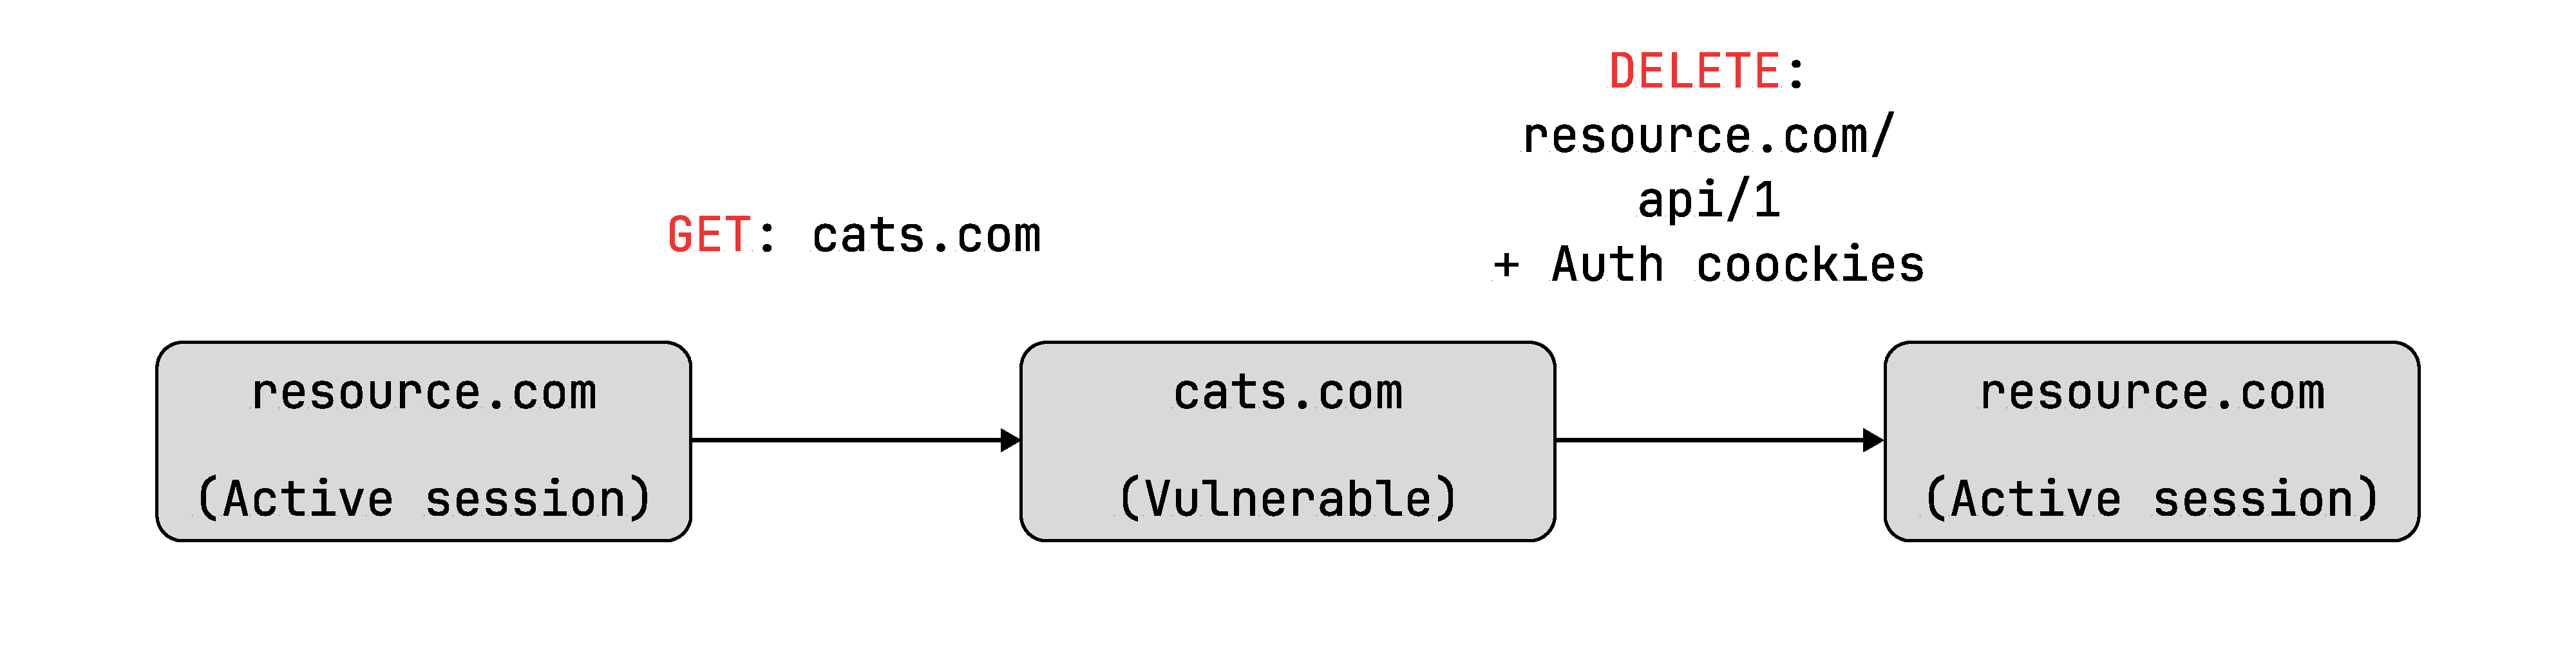
\includegraphics[width=1\textwidth]{img/Csrf_diagram}
    ~\caption{CSRF attack principle diagram.}\label{fig:csrf_diagram}
\end{figure}

Файлы cookie имеют параметр \texttt{SameSite}, который определяет будут ли они отправлены вместе с запросом на сайт,
имеющим другой домен.

Существует три возможных значения параметра \texttt{SameSite}:

\begin{itemize}
    \item \textbf{None} - прямо указывает, что на передачу cookie-файлов не накладывается никаких ограничений.
    \item \textbf{Lax} - разрешает передачу cookie только безопасными HTTP-методами, которыми, согласно
    RFC 7231~\cite{fielding2014rfc}, являются \texttt{GET, HEAD, OPTIONS} и \texttt{TRACE}.
    \item \textbf{Strict} - является самым строгим вариантом безопасности и блокирует отправку cookie с любыми
    запросами на сайт под другим доменом.
    Файлы cookie будут передаваться только в пределах того домена, с которого они и были установлены.
\end{itemize}

Таким образом, значения параметра \texttt{SameSite} такие как \texttt{Lax} и \texttt{Strict} защищают пользователя
от CSRF-атаки, так как блокируют прикрепление файлов cookie к запросу, что был инициирован ресурсом злоумышленника.

Другие методы защиты от CSRF описаны в~\cite{owaspCsrf}.